% Options for packages loaded elsewhere
\PassOptionsToPackage{unicode}{hyperref}
\PassOptionsToPackage{hyphens}{url}
\PassOptionsToPackage{dvipsnames,svgnames,x11names}{xcolor}
%
\documentclass[
  12pt,
]{article}

\usepackage{amsmath,amssymb}
\usepackage{setspace}
\usepackage{iftex}
\ifPDFTeX
  \usepackage[T1]{fontenc}
  \usepackage[utf8]{inputenc}
  \usepackage{textcomp} % provide euro and other symbols
\else % if luatex or xetex
  \usepackage{unicode-math}
  \defaultfontfeatures{Scale=MatchLowercase}
  \defaultfontfeatures[\rmfamily]{Ligatures=TeX,Scale=1}
\fi
\usepackage{lmodern}
\ifPDFTeX\else  
    % xetex/luatex font selection
  \setmainfont[]{Times New Roman}
\fi
% Use upquote if available, for straight quotes in verbatim environments
\IfFileExists{upquote.sty}{\usepackage{upquote}}{}
\IfFileExists{microtype.sty}{% use microtype if available
  \usepackage[]{microtype}
  \UseMicrotypeSet[protrusion]{basicmath} % disable protrusion for tt fonts
}{}
\makeatletter
\@ifundefined{KOMAClassName}{% if non-KOMA class
  \IfFileExists{parskip.sty}{%
    \usepackage{parskip}
  }{% else
    \setlength{\parindent}{0pt}
    \setlength{\parskip}{6pt plus 2pt minus 1pt}}
}{% if KOMA class
  \KOMAoptions{parskip=half}}
\makeatother
\usepackage{xcolor}
\usepackage[margin=2cm]{geometry}
\setlength{\emergencystretch}{3em} % prevent overfull lines
\setcounter{secnumdepth}{5}
% Make \paragraph and \subparagraph free-standing
\ifx\paragraph\undefined\else
  \let\oldparagraph\paragraph
  \renewcommand{\paragraph}[1]{\oldparagraph{#1}\mbox{}}
\fi
\ifx\subparagraph\undefined\else
  \let\oldsubparagraph\subparagraph
  \renewcommand{\subparagraph}[1]{\oldsubparagraph{#1}\mbox{}}
\fi


\providecommand{\tightlist}{%
  \setlength{\itemsep}{0pt}\setlength{\parskip}{0pt}}\usepackage{longtable,booktabs,array}
\usepackage{calc} % for calculating minipage widths
% Correct order of tables after \paragraph or \subparagraph
\usepackage{etoolbox}
\makeatletter
\patchcmd\longtable{\par}{\if@noskipsec\mbox{}\fi\par}{}{}
\makeatother
% Allow footnotes in longtable head/foot
\IfFileExists{footnotehyper.sty}{\usepackage{footnotehyper}}{\usepackage{footnote}}
\makesavenoteenv{longtable}
\usepackage{graphicx}
\makeatletter
\def\maxwidth{\ifdim\Gin@nat@width>\linewidth\linewidth\else\Gin@nat@width\fi}
\def\maxheight{\ifdim\Gin@nat@height>\textheight\textheight\else\Gin@nat@height\fi}
\makeatother
% Scale images if necessary, so that they will not overflow the page
% margins by default, and it is still possible to overwrite the defaults
% using explicit options in \includegraphics[width, height, ...]{}
\setkeys{Gin}{width=\maxwidth,height=\maxheight,keepaspectratio}
% Set default figure placement to htbp
\makeatletter
\def\fps@figure{htbp}
\makeatother
% definitions for citeproc citations
\NewDocumentCommand\citeproctext{}{}
\NewDocumentCommand\citeproc{mm}{%
  \begingroup\def\citeproctext{#2}\cite{#1}\endgroup}
\makeatletter
 % allow citations to break across lines
 \let\@cite@ofmt\@firstofone
 % avoid brackets around text for \cite:
 \def\@biblabel#1{}
 \def\@cite#1#2{{#1\if@tempswa , #2\fi}}
\makeatother
\newlength{\cslhangindent}
\setlength{\cslhangindent}{1.5em}
\newlength{\csllabelwidth}
\setlength{\csllabelwidth}{3em}
\newenvironment{CSLReferences}[2] % #1 hanging-indent, #2 entry-spacing
 {\begin{list}{}{%
  \setlength{\itemindent}{0pt}
  \setlength{\leftmargin}{0pt}
  \setlength{\parsep}{0pt}
  % turn on hanging indent if param 1 is 1
  \ifodd #1
   \setlength{\leftmargin}{\cslhangindent}
   \setlength{\itemindent}{-1\cslhangindent}
  \fi
  % set entry spacing
  \setlength{\itemsep}{#2\baselineskip}}}
 {\end{list}}
\usepackage{calc}
\newcommand{\CSLBlock}[1]{\hfill\break\parbox[t]{\linewidth}{\strut\ignorespaces#1\strut}}
\newcommand{\CSLLeftMargin}[1]{\parbox[t]{\csllabelwidth}{\strut#1\strut}}
\newcommand{\CSLRightInline}[1]{\parbox[t]{\linewidth - \csllabelwidth}{\strut#1\strut}}
\newcommand{\CSLIndent}[1]{\hspace{\cslhangindent}#1}

\usepackage[noblocks]{authblk}
\renewcommand*{\Authsep}{, }
\renewcommand*{\Authand}{, }
\renewcommand*{\Authands}{, }
\renewcommand\Affilfont{\small}
\usepackage{threeparttable}
\makeatletter
\@ifpackageloaded{caption}{}{\usepackage{caption}}
\AtBeginDocument{%
\ifdefined\contentsname
  \renewcommand*\contentsname{Table of contents}
\else
  \newcommand\contentsname{Table of contents}
\fi
\ifdefined\listfigurename
  \renewcommand*\listfigurename{List of Figures}
\else
  \newcommand\listfigurename{List of Figures}
\fi
\ifdefined\listtablename
  \renewcommand*\listtablename{List of Tables}
\else
  \newcommand\listtablename{List of Tables}
\fi
\ifdefined\figurename
  \renewcommand*\figurename{Figure}
\else
  \newcommand\figurename{Figure}
\fi
\ifdefined\tablename
  \renewcommand*\tablename{Table}
\else
  \newcommand\tablename{Table}
\fi
}
\@ifpackageloaded{float}{}{\usepackage{float}}
\floatstyle{ruled}
\@ifundefined{c@chapter}{\newfloat{codelisting}{h}{lop}}{\newfloat{codelisting}{h}{lop}[chapter]}
\floatname{codelisting}{Listing}
\newcommand*\listoflistings{\listof{codelisting}{List of Listings}}
\makeatother
\makeatletter
\makeatother
\makeatletter
\@ifpackageloaded{caption}{}{\usepackage{caption}}
\@ifpackageloaded{subcaption}{}{\usepackage{subcaption}}
\makeatother
\ifLuaTeX
  \usepackage{selnolig}  % disable illegal ligatures
\fi
\usepackage{bookmark}

\IfFileExists{xurl.sty}{\usepackage{xurl}}{} % add URL line breaks if available
\urlstyle{same} % disable monospaced font for URLs
\hypersetup{
  pdftitle={Perceptions of Inequality and Meritocracy: Their Interplay in Shaping Preferences for Market Justice in Chile (2016-2023)},
  pdfauthor={Equipo EDUMER},
  colorlinks=true,
  linkcolor={blue},
  filecolor={Maroon},
  citecolor={Blue},
  urlcolor={Blue},
  pdfcreator={LaTeX via pandoc}}

\title{Perceptions of Inequality and Meritocracy: Their Interplay in
Shaping Preferences for Market Justice in Chile (2016-2023)}


  \author{Juan Carlos Castillo}
            \affil{%
                  Departamento de Sociología, Universidad de Chile
              }
          \affil{%
                  Centro de estudios del conflicto y cohesión social
                  (COES)
              }
          \affil{%
                  Núcleo milenio de desigualdades y oportunidades
                  digitales (NUDOS)
              }
        \author{Andreas Laffert}
            \affil{%
                  Instituto de Sociología, Pontificia Universidad
                  Católica de Chile
              }
        \author{Kevin Carrasco}
            \affil{%
                  Centro de estudios del conflicto y cohesión social
                  (COES)
              }
        \author{Julio Iturra}
            \affil{%
                  International Graduate School of Social Sciencies
                  (BIGSSS), University of Bremen, Germany
              }
      
\date{}
\begin{document}
\maketitle
\begin{abstract}
My abstract. \newline \textbf{Keywords}: meritocracy, social inequality,
inequality justification, COVID-19
\end{abstract}

\setstretch{1.15}
\section{Introduction}\label{introduction}

Since 1980, economic inequality and wealth concentration have
dramatically increased worldwide, becoming one of the main challenges
for the social sciences. Globally, in 2021, less than 50\% of the world
population owned only 2\% of the wealth, while the richest 10\%
concentrated 76\%, and the wealthiest 1\% captured nearly 38\% of total
assets (\citeproc{ref-chancel_world_2022}{Chancel et al., 2022}). This
context of economic disparity has sparked renewed interest in studying
not only the objective aspects of inequality, such as income and access
to resources, but also its subjective dimensions, including perceptions,
beliefs, and associated attitudes
(\citeproc{ref-janmaat_subjective_2013}{Janmaat, 2013}). This has led,
among other reasons, to widespread concern in the social sciences about
the political delegitimization that economic inequality can produce
(\citeproc{ref-castillo_perception_2022}{Castillo et al., 2022}).
Understanding how people perceive inequality is crucial, as these
perceptions can influence how societies comprehend and justify the
distribution of goods and services.

The perception of economic inequality can be understood as an
individual's subjective assessment of how resources are allocated among
members of a given society (\citeproc{ref-akyelken_urban_2020}{Akyelken,
2020}). Regardless of their measurement, various studies have shown that
this perception often underestimates the gap between the rich and the
poor, which could have implications for attitudes toward the
distribution of goods and services
(\citeproc{ref-castillo_perception_2022}{Castillo et al., 2022};
\citeproc{ref-schroder_income_2017}{Schröder, 2017}). Moreover, in
recent years, there has been a discussion about the subjective and
objective aspects of inequality, demonstrating inconsistencies between
the two (\citeproc{ref-trump_income_2018}{Trump, 2018}). This tension is
relevant because advancing the study of perceptions could help
understand how perceived inequality affects the distribution of
resources within a society (Becker, 2020).

Perception of economic inequality has been associated with important
outcomes such as redistributive preferences, justification of
inequality, and legitimacy of the economic system (Castillo et al., 2022
{[}acá citar gente de Granada{]}). Research shows that greater perceived
inequality fosters stronger preferences for redistribution, regardless
of actual inequality levels
(\citeproc{ref-garcia-sanchez_vicious_2019}{García-Sánchez et al.,
2019}; \citeproc{ref-gimpelson_misperceiving_2018}{Gimpelson \&
Treisman, 2018}). However, other findings suggest that heightened
perceptions of income gaps between high- and low-paying occupations may
lead to greater justification of inequality
(\citeproc{ref-Castillo2011}{Castillo, 2011}). A less explored area in
this regard concerns market justice, which denotes the degree to which
individuals consider just that social goods and services (e.g., health,
pensions, education) are allocated according to individual contribution,
competition, and ability to pay
(\citeproc{ref-kluegel_legitimation_1999}{Kluegel et al., 1999};
\citeproc{ref-lane_market_1986}{Lane, 1986};
\citeproc{ref-lindh_public_2015}{Lindh, 2015}). Market justice attitudes
reflect the belief that the market promotes procedural
fairness---equality of opportunity---so that outcomes result from
individual achievement (\citeproc{ref-lane_market_1986}{Lane, 1986}).
Indeed, Lindh (\citeproc{ref-lindh_public_2015}{2015}) shows that market
justice preferences are stronger in countries with higher private
spending on services than in those with more comprehensive welfare
systems. From this perspective, perceptions of economic inequality may
be key, as lower perceived gaps can reinforce acceptance of free-market
systems and justify existing inequalities.

Meritocracy posits that inequality is an inherent feature of societies
but can be legitimized through fairer principles, such as effort and
talent (\citeproc{ref-davis_principles_2001}{Davis \& Moore, 2001};
\citeproc{ref-young_rise_1962}{Young, 1962}). Previous studies have
demonstrated that people with stronger meritocratic beliefs tend to
perceive less inequality as they attribute economic differences to
individual achievements (\citeproc{ref-mijs_paradox_2021}{Mijs, 2021};
\citeproc{ref-wilson_role_2003}{Wilson, 2003}) and also to justify more
inequality since these beliefs are associated with attitudes that
maintain the legitimization of social differences
(\citeproc{ref-batruch_belief_2023}{Batruch et al., 2023}). In a context
like Chile, where the distribution of goods and services is
predominantly governed by market logics strongly introduced during the
military dictatorship (1973-1989)
(\citeproc{ref-boccardo_30_2020}{Boccardo, 2020}), these beliefs can
play a crucial role in the acceptance of social inequalities.
Incorporating the perception of meritocracy in this literature allows
for an understanding of how attitudes toward inequality are shaped not
only by the perception of economic gaps, but also by beliefs about how
these gaps are justified. Furthermore, these beliefs are often
consolidated from an early age, reinforced by institutions promoting
values such as effort and individual skills to climb socially
(\citeproc{ref-castillo_socialization_2024}{Castillo et al., 2024};
\citeproc{ref-reynolds_perceptions_2014}{Reynolds \& Xian, 2014}).

The perception of meritocracy and the perception of economic inequality
would interact intricately in shaping preferences for market justice. On
the one hand, a stronger perception of merit as a criterion for
distribution could minimize the perception of economic gaps, thus
justifying an unequal system
(\citeproc{ref-castillo_percepcion_2019}{Castillo et al., 2012};
\citeproc{ref-mijs_paradox_2021}{Mijs, 2021}). On the other hand, the
perception of inequality could moderate the impact of meritocracy, as a
higher perception of economic gaps might challenge the idea that these
are solely based on merit.

The primary objective of this study is to analyze the interplay between
perceptions of inequality and meritocracy and their joint influence on
preferences for market justice in Chile from 2016 to 2023, using
longitudinal data from the ELSOC survey. This interaction is expected to
provide a more comprehensive explanation of attitudes toward market
justice in a country characterized by high inequality and strong
free-market influence (\citeproc{ref-boccardo_30_2020}{Boccardo, 2020};
\citeproc{ref-flores_top_2020}{Flores et al., 2020}). Additionally, this
analysis seeks to elucidate how political and social
contingencies---such as the 2019 and 2022 social movements---might have
moderated these relationships by prompting more critical reflection on
the commodification of social services. Recognizing the temporal
dimension in shaping market justice preferences is essential, given that
such preferences are not static but are influenced by historical and
contextual factors that challenge or reaffirm prevailing social norms.
In this regard, variations in perceived economic inequality and
meritocracy over time can affect how individuals endorse market-based
approaches. Consequently, public opinion may shift from supporting
market justice to embracing redistributive policies aimed at mitigating
inequalities.

\section{Theoretical views on market justice, inequality perception and
meritocracy}\label{theoretical-views-on-market-justice-inequality-perception-and-meritocracy}

\subsection{Justification of market
inequality}\label{justification-of-market-inequality}

Market justice has been discussed in the literature as a normative
principle that legitimates the distribution of economic rewards based on
individual merit and effort. The most detailed theoretical account of
this concept is provided by Lane
(\citeproc{ref-lane_market_1986}{1986}), who defines market justice as a
system of ``earned deserts,'' whereby individuals are seen as entitled
to their outcomes insofar as these are a product of personal
productivity and competition. This view directly contrasts with
political justice, which emphasizes redistributive mechanisms based on
the principles of equality and need, and is often materialized through
welfare policies. For Lane (\citeproc{ref-lane_market_1986}{1986}),
market justice relies on the conception that markets are neutral and
self-regulating arenas, where individuals are treated fairly because
they face the same formal rules of engagement. What matters is not
whether everyone ends up with the same, but that everyone has the chance
to compete, and that success reflects effort and ability. Consequently,
the legitimacy of market justice stems from the assumption that
inequalities are not only inevitable but fair---so long as the rules are
transparent and opportunities are open. These beliefs align with a
broader ideological framework that values individual autonomy, private
property, and limited government intervention. In this way, market
justice provides a moral justification for inequality by framing it as a
necessary outcome of personal responsibility and societal efficiency.

Empirical studies have developed different strategies to capture and
operationalize market justice preferences. A common approach in the
literature is to gauge attitudes toward the legitimacy of inequality in
specific domains, especially when linked to income differences. Kluegel
and Smith (\citeproc{ref-kluegel_beliefs_1981}{1981}) and later Kluegel
et al. (\citeproc{ref-kluegel_legitimation_1999}{1999}) laid the
groundwork for measuring beliefs in market justice through survey items
that assess whether people support economic inequality when it reflects
personal effort and skill. Over time, this approach has been extended
beyond income to include other market-mediated outcomes, such as
education, healthcare, or pensions. For example, Knesebeck et al.~(2016)
and Immergut and Schneider (\citeproc{ref-immergut_it_2020}{2020})
examine whether citizens consider it fair that individuals with higher
incomes can access better healthcare, while Lee and Stacey
(\citeproc{ref-lee_fairness_2023}{2023}) apply a similar method in the
context of education in Australia. These studies usually rely on a
survey item asking respondents to evaluate the fairness of income-based
access to welfare services, allowing for comparing justice perceptions
across different contexts. Some research, like that of Lindh
(\citeproc{ref-lindh_public_2015}{2015}) and Svallfors
(\citeproc{ref-svallfors_political_2007}{2007}), uses these indicators
in combination to measure broader preferences for market-based
distribution in welfare systems. More recently, Castillo et al.
(\citeproc{ref-castillo_socialization_2024}{2024}) introduced a
single-item composite measure of market justice to assess student
attitudes toward income-based access to education, healthcare, and
pensions in Chile. These different operationalizations all aim to
capture the extent to which individuals accept inequality when it is
framed as a reflection of market outcomes.

The study of market justice preferences has increasingly focused on how
they are shaped by individuals' socioeconomic position, normative
beliefs, and the institutional context in which they are embedded.
Across the literature, there is strong empirical evidence suggesting
that individuals in more advantaged socioeconomic positions---those with
higher income, education, and occupational status---are more likely to
endorse market-based distribution as fair and legitimate
(\citeproc{ref-koos_moral_2019}{Koos \& Sachweh, 2019};
\citeproc{ref-svallfors_political_2007}{Svallfors, 2007}). This tendency
reflects not only material self-interest but also a broader moral
economy, in which winners of the market system internalize
justifications for the status quo. At the same time, normative and
ideological orientations---such as conservative, liberal, or neoliberal
values---are consistently associated with greater support for
meritocratic principles and skepticism toward redistribution. This is
particularly visible in contexts such as Chile and Australia, where
studies by Castillo et al.
(\citeproc{ref-castillo_socialization_2024}{2024}) and Lee and Stacey
(\citeproc{ref-lee_fairness_2023}{2023}) show that those with
right-leaning political preferences tend to view income-based access to
welfare services as legitimate. Beyond individual-level characteristics,
country-level institutions also play a central role. In liberal welfare
regimes like those of the United States or the United Kingdom, market
justice preferences are more widespread, while in coordinated or
social-democratic regimes---such as Sweden or Germany---citizens are
generally more critical of market-based inequalities
(\citeproc{ref-immergut_it_2020}{Immergut \& Schneider, 2020};
\citeproc{ref-lindh_public_2015}{Lindh, 2015}). These findings suggest
that market justice is not a fixed belief but a contextually shaped
orientation, mediated by structural conditions, cultural values, and the
historical development of welfare institutions.

\subsection{Perception of inequality}\label{perception-of-inequality}

Perceptions of inequality refer to individuals' subjective evaluations
of the extent, causes, and consequences of income and wealth
disparities. Unlike objective measures such as the Gini index, perceived
inequality captures how individuals make sense of distributive
hierarchies in their everyday lives, shaped by reference groups, social
comparisons, and information environments
(\citeproc{ref-garcia-castro_perceiving_2020}{García-Castro et al.,
2020}; \citeproc{ref-gimpelson_misperceiving_2018}{Gimpelson \&
Treisman, 2018}; \citeproc{ref-mijs_stratified_2016}{Mijs, 2016}).
Scholars have proposed multiple dimensions of perceived inequality,
including its magnitude (how significant are the gaps), vertical
structure (between which groups), trend over time (increasing or
decreasing), and legitimacy (whether it is just or not)
(\citeproc{ref-engelhardt_what_2018}{Engelhardt \& Wagener, 2018};
\citeproc{ref-garcia-sanchez_vicious_2019}{García-Sánchez et al.,
2019}). These dimensions encompass both cognitive and normative aspects
of perceptions of inequality and can vary across societies and social
groups, depending on exposure, ideology, and personal experience
(\citeproc{ref-castillo_perception_2022}{Castillo et al., 2022};
\citeproc{ref-garcia-sanchez_perceptions_2018}{García-Sánchez et al.,
2018}).

Among the different approaches to measuring perceived inequality, one of
the most widely used is the estimation of wage gaps between occupational
extremes, such as between a CEO and a manual worker. This type of item
provides a concrete frame that respondents can relate to more easily
than abstract questions about national income distribution {[}Castillo
et al. (\citeproc{ref-castillo_percepcion_2019}{2012}); Easterbrook
(\citeproc{ref-easterbrook_social_2021}{2021}); Willis et al., 2015{]}.
While it enables the estimation of inequality using simple heuristics,
this method is not without challenges. For instance, people often lack
reliable knowledge about the earnings of those at the top of the income
ladder, which leads to high variability in responses and the use of
biased mental shortcuts (\citeproc{ref-knell_perceptions_2020}{Knell \&
Stix, 2020}). Despite this, perceived wage gaps are strong predictors of
political
attitudes(\citeproc{ref-garcia-sanchez_perceptions_2018}{García-Sánchez
et al., 2018}; \citeproc{ref-pedersen_attitudes_2019}{Pedersen \& Mutz,
2019}), making them a valuable tool for understanding public responses
to economic disparities.

Another relevant critique of this approach lies in its conflation of
different psychological constructs. Many surveys assess perceived
inequality through Likert-type items that ask respondents to agree or
disagree with statements, such as ``income differences are too large,''
which captures general concern or discomfort rather than a specific
perception (\citeproc{ref-Castillo2011}{Castillo, 2011};
\citeproc{ref-garcia-sanchez_vicious_2019}{García-Sánchez et al.,
2019}).These items mix cognitive estimations with affective evaluations,
complicating the interpretation of what respondents perceive versus what
they morally reject. As a result, the conceptual clarity between
perceived inequality and inequality aversion remains blurred in many
empirical studies. To address this limitation, recent work has
emphasized the need to distinguish between absolute and comparative
measures, as well as between ideal and actual estimates of economic gaps
{[}García-Sánchez \& De Carvalho
(\citeproc{ref-garcia-sanchez_creencias_2022}{2022}); Auspurg et al.,
2017{]}.

Importantly, perceptions of inequality have been linked to attitudes
about market justice---the belief that goods and services should be
allocated according to individual contribution, competition, or
willingness to pay (\citeproc{ref-kluegel_social_1995a}{Kluegel et al.,
1995}; \citeproc{ref-lindh_public_2015}{Lindh, 2015}). Research
indicates that lower perceived inequality can reinforce support for
market-based distributive arrangements by suggesting that the system is
fair and that outcomes reflect effort and ability
(\citeproc{ref-kuhn_eye_2011}{Kuhn, 2011}). In contrast, when inequality
is perceived as excessive or structurally determined, individuals could
question the legitimacy of market justice and become more supportive of
redistributive policies
(\citeproc{ref-castillo_perception_2022}{Castillo et al., 2022};
\citeproc{ref-garcia-sanchez_vicious_2019}{García-Sánchez et al.,
2019}).

\subsection{Perception of meritocracy}\label{perception-of-meritocracy}

Meritocracy constitutes a central ideological framework for legitimizing
social inequality. Rooted in the belief that rewards and positions
should be allocated based on individual effort and talent, meritocracy
operates as a normative ideal and a descriptive belief about how society
functions. As initially conceptualized by Michael Young
(\citeproc{ref-young_rise_1962}{1962}), the term was meant to critique a
system in which merit-based stratification becomes a new form of
inequality. However, over time, meritocracy has been widely adopted in
many societies as a fair and desirable principle of distribution,
particularly within liberal democracies and market-oriented economies
(\citeproc{ref-mijs_paradox_2021}{Mijs, 2021};
\citeproc{ref-sandel_tyranny_2020}{Sandel, 2020}). From a sociological
perspective, the belief in meritocracy is more than a cognitive
assessment; it reflects a moral lens through which individuals interpret
inequality. People who believe that success results from hard work and
talent are more likely to view social and economic disparities as
legitimate (\citeproc{ref-batruch_belief_2023}{Batruch et al., 2023};
\citeproc{ref-castillo_percepcion_2019}{Castillo et al., 2012}).
Conversely, if they see outcomes as driven by luck, social origin, or
systemic barriers, inequality is more likely to be perceived as unjust.
This distinction becomes crucial in societies with persistent structural
inequality, where public narratives often emphasize personal
responsibility and merit while overlooking entrenched disadvantages.

We adopt a multidimensional perspective on meritocracy, distinguishing
between two key dimensions: effort-based and talent-based perceptions.
This distinction is essential, as it captures different pathways through
which individuals justify inequality. Effort-based meritocracy
emphasizes hard work and perseverance as the basis for social rewards,
aligning closely with cultural narratives of personal responsibility. A
talent-based meritocracy, by contrast, emphasizes intelligence and
innate abilities, which are often perceived as less malleable and more
unequally distributed. Both dimensions have been shown to correlate with
acceptance of inequality, but they may carry distinct implications for
how inequality is justified in specific domains
(\citeproc{ref-castillo_multidimensional_2023}{Castillo et al., 2023}).
The relevance of this distinction is supported by recent studies, which
show that individuals respond differently to these dimensions. For
instance, perceptions that effort is rewarded in society are more
strongly associated with positive evaluations of fairness and acceptance
of unequal outcomes (\citeproc{ref-batruch_belief_2023}{Batruch et al.,
2023}). This may be because effort is seen as a controllable and morally
virtuous trait, whereas talent is often perceived as a natural
advantage. Consequently, effort-based meritocracy is likely more potent
in legitimizing inequality, particularly in neoliberal contexts.

These dimensions of meritocracy reflect how respondents perceive
society's distributive logic, regardless of whether they personally
endorse meritocratic principles. This distinction aligns with recent
findings indicating that individuals distinguish between how merit is
perceived in society and how it should ideally operate, which in turn
shapes their preferences for redistribution and justice
(Tejero-Peregrina et al., 2025). Meritocratic beliefs serve as symbolic
justifications for unequal outcomes, particularly when access is
stratified by income or social opportunity. Prior studies have shown
that individuals who perceive higher levels of meritocracy tend to
express stronger support for unequal distributions that reflect market
outcomes (\citeproc{ref-castillo_percepcion_2019}{Castillo et al.,
2012}; \citeproc{ref-castillo_socialization_2024}{Castillo et al.,
2024}).

In addition to influencing individual attitudes toward inequality,
meritocratic beliefs can contribute to social division and the
stigmatization of disadvantaged groups. Recent research has demonstrated
that exposure to meritocratic narratives can reinforce the belief that
poverty results from individual failings rather than systemic
conditions, reducing support for redistributive measures and increasing
the stigmatization of the poor (Hoyt \& Burnette, 2023). This reinforces
negative stereotypes and reduces empathy toward individuals from lower
socioeconomic backgrounds. Moreover, Busemeyer, Abrassart, and Nezi
(2019) argue that meritocratic narratives can serve as feedback
mechanisms that shape public opinion and well-being by framing
individuals' understanding of welfare outcomes as deserved or undeserved
within existing institutional structures. This psychological mechanism
highlights the normative power of meritocracy in stabilizing unequal
systems by shaping political attitudes and personal perceptions of
success and failure.

\subsection{This study (hypotheses)}\label{this-study-hypotheses}

\section{Data, Variables and Methods}\label{data-variables-and-methods}

\subsection{Data}\label{data}

This study draws on data from the Chilean Longitudinal Social Survey
(ELSOC), a panel study collected annually from 2016 to 2023. The survey
evaluates how individuals think, feel, and behave regarding conflict and
social cohesion in Chile. ELSOC employs a probabilistic, stratified,
clustered, multistage sampling design encompassing major urban centers
(Santiago, Valparaíso, and Concepción) and smaller cities. The target
population includes women and men aged 18--75 who are habitual residents
of private dwellings. The first wave included 2,927 participants,
representing northern and southern regions, covering 77\% of the
country's total population and 93\% of its urban population, with a
response rate of 62.4\% (\citeproc{ref-elsoc_estudio_2022}{ELSOC,
2022}).

The survey has been conducted yearly since 2016, except in 2020, when it
was suspended due to the pandemic. Waves 2016, 2017, 2018, 2019, 2022,
and 2023 used computer-assisted personal interviewing (CAPI), while a
reduced wave in 2021 employed computer-assisted telephone interviews
(CATI). Wave 3 included a refreshment sample (N = 1,519) to counter
attrition, but these cases are not used here to capture longer response
trends. Between wave 1 and wave 7, attrition amounted to 40\%, achieving
a final sample of N = 1,741. Longitudinal weights adjust for both the
sampling design and potential biases arising from systematic
non-participation. Further details on sampling, attrition, and weighting
can be found at \url{https://coes.cl/encuesta-panel/}, and the dataset
is publicly available at
\url{https://dataverse.harvard.edu/dataverse/elsoc}.

\subsection{Variables}\label{variables}

\emph{Dependent variable}

\textbf{Market justice preferences}: The dependent variable in this
study is preferences for market justice. This construct is
operationalized through three items that capture how strongly
individuals justify conditioning access to social services---healthcare,
pensions, and education---on income. Specifically, the justification of
inequality in healthcare is assessed by the question: ``Is it fair in
Chile that people with higher incomes can access better healthcare than
people with lower incomes?'' The same question is posed for pensions and
education. In all cases, respondents indicate their level of agreement
on a five-point Likert scale ranging from 1 (``strongly disagree'') to 5
(``strongly agree''). Additionally, we include a composite measure of
``market justice preferences'', calculated as the average of these three
items (\(\alpha\) = 0.84). This index ranges from 1 to 5, with higher
values indicating stronger preferences for market justice (see
Table~\ref{tbl-summary1}).

\begin{longtable}[]{@{}
  >{\raggedright\arraybackslash}p{(\columnwidth - 6\tabcolsep) * \real{0.3367}}
  >{\raggedright\arraybackslash}p{(\columnwidth - 6\tabcolsep) * \real{0.3367}}
  >{\raggedright\arraybackslash}p{(\columnwidth - 6\tabcolsep) * \real{0.2143}}
  >{\raggedright\arraybackslash}p{(\columnwidth - 6\tabcolsep) * \real{0.1122}}@{}}
\caption{Dependent variables for the first wave
(2016)}\label{tbl-summary1}\tabularnewline
\toprule\noalign{}
\begin{minipage}[b]{\linewidth}\raggedright
Label
\end{minipage} & \begin{minipage}[b]{\linewidth}\raggedright
Stats / Values
\end{minipage} & \begin{minipage}[b]{\linewidth}\raggedright
Freqs (\% of Valid)
\end{minipage} & \begin{minipage}[b]{\linewidth}\raggedright
Valid
\end{minipage} \\
\midrule\noalign{}
\endfirsthead
\toprule\noalign{}
\begin{minipage}[b]{\linewidth}\raggedright
Label
\end{minipage} & \begin{minipage}[b]{\linewidth}\raggedright
Stats / Values
\end{minipage} & \begin{minipage}[b]{\linewidth}\raggedright
Freqs (\% of Valid)
\end{minipage} & \begin{minipage}[b]{\linewidth}\raggedright
Valid
\end{minipage} \\
\midrule\noalign{}
\endhead
\bottomrule\noalign{}
\endlastfoot
Health distributive justice &
\begin{minipage}[t]{\linewidth}\raggedright
1. Strongly desagree\\
2. Desagree\\
3. Neither agree nor desagre\\
4. Agree\\
5. Strongly agree\strut
\end{minipage} & \begin{minipage}[t]{\linewidth}\raggedright
554 (37.5\%)\\
713 (48.3\%)\\
61 ( 4.1\%)\\
131 ( 8.9\%)\\
18 ( 1.2\%)\strut
\end{minipage} & \begin{minipage}[t]{\linewidth}\raggedright
1477\\
(100.0\%)\strut
\end{minipage} \\
Pension distributive justice &
\begin{minipage}[t]{\linewidth}\raggedright
1. Strongly desagree\\
2. Desagree\\
3. Neither agree nor desagre\\
4. Agree\\
5. Strongly agree\strut
\end{minipage} & \begin{minipage}[t]{\linewidth}\raggedright
425 (28.8\%)\\
704 (47.7\%)\\
106 ( 7.2\%)\\
219 (14.8\%)\\
23 ( 1.6\%)\strut
\end{minipage} & \begin{minipage}[t]{\linewidth}\raggedright
1477\\
(100.0\%)\strut
\end{minipage} \\
Education distributive justice &
\begin{minipage}[t]{\linewidth}\raggedright
1. Strongly desagree\\
2. Desagree\\
3. Neither agree nor desagre\\
4. Agree\\
5. Strongly agree\strut
\end{minipage} & \begin{minipage}[t]{\linewidth}\raggedright
519 (35.1\%)\\
764 (51.7\%)\\
71 ( 4.8\%)\\
112 ( 7.6\%)\\
11 ( 0.7\%)\strut
\end{minipage} & \begin{minipage}[t]{\linewidth}\raggedright
1477\\
(100.0\%)\strut
\end{minipage} \\
Market justice preferences & \begin{minipage}[t]{\linewidth}\raggedright
Mean (sd) : 2 (0.8)\\
min \textless{} med \textless{} max:\\
1 \textless{} 2 \textless{} 5\\
IQR (CV) : 1 (0.4)\strut
\end{minipage} & 12 distinct values &
\begin{minipage}[t]{\linewidth}\raggedright
1477\\
(100.0\%)\strut
\end{minipage} \\
\end{longtable}

\emph{Independent variables}

\textbf{Perception of economic inequality}: The main independent
variable refers to the perception of economic inequality, measured
through the perceived wage gap, which serves as an absolute indicator of
inequality perceptions (\citeproc{ref-castillo_perception_2022}{Castillo
et al., 2022}). This measure is derived from the gap between the
perceived salaries of jobs at opposite ends of the occupational
hierarchy. Specifically, it relies on the logarithm of the division
between the perceived salary of a large-company president and that of an
unskilled worker (\citeproc{ref-Castillo2011}{Castillo, 2011}). Higher
values of this term indicate a greater perception of economic inequality
between occupations located at the extremes of the status continuum.

\textbf{Justification of economic inequality}: This construct is
measured as the just earnings gap, an approach to measuring the
justification of economic inequality based on earning differences
considered just between high and low status occupations
(\citeproc{ref-Castillo2011}{Castillo, 2011}). Similarly to economic
inequality perception, this indicator relies on the logarithmic ratio
between the just salary of a large-company president and that of an
unskilled worker. Higher values of this term indicate a greater
justification of economic inequality.

\textbf{Meritocracy}: Meritocratic perception is operationalized through
two components: one addressing effort and another focusing on talent
(\citeproc{ref-young_rise_1962}{Young, 1962}). The item used to gauge
effort is: ``In Chile, people are rewarded for their efforts,'' while
the item for talent is: ``In Chile, people are rewarded for their
intelligence and skills.'' In both cases, respondents indicate their
level of agreement on a five-point Likert scale, ranging from 1
(``strongly disagree'') to 5 (``strongly agree'').

Table 2 shows the independent variables used, their response categories
and their frequencies.

\begin{longtable}[]{@{}
  >{\raggedright\arraybackslash}p{(\columnwidth - 6\tabcolsep) * \real{0.3774}}
  >{\raggedright\arraybackslash}p{(\columnwidth - 6\tabcolsep) * \real{0.3113}}
  >{\raggedright\arraybackslash}p{(\columnwidth - 6\tabcolsep) * \real{0.2075}}
  >{\raggedright\arraybackslash}p{(\columnwidth - 6\tabcolsep) * \real{0.1038}}@{}}
\caption{Independent variables for the first wave
(2016)}\label{tbl-summary2}\tabularnewline
\toprule\noalign{}
\begin{minipage}[b]{\linewidth}\raggedright
Label
\end{minipage} & \begin{minipage}[b]{\linewidth}\raggedright
Stats / Values
\end{minipage} & \begin{minipage}[b]{\linewidth}\raggedright
Freqs (\% of Valid)
\end{minipage} & \begin{minipage}[b]{\linewidth}\raggedright
Valid
\end{minipage} \\
\midrule\noalign{}
\endfirsthead
\toprule\noalign{}
\begin{minipage}[b]{\linewidth}\raggedright
Label
\end{minipage} & \begin{minipage}[b]{\linewidth}\raggedright
Stats / Values
\end{minipage} & \begin{minipage}[b]{\linewidth}\raggedright
Freqs (\% of Valid)
\end{minipage} & \begin{minipage}[b]{\linewidth}\raggedright
Valid
\end{minipage} \\
\midrule\noalign{}
\endhead
\bottomrule\noalign{}
\endlastfoot
Inequality gap perception & \begin{minipage}[t]{\linewidth}\raggedright
Mean (sd) : 3.7 (1.1)\\
min \textless{} med \textless{} max:\\
0.4 \textless{} 3.7 \textless{} 6.9\\
IQR (CV) : 1.6 (0.3)\strut
\end{minipage} & 294 distinct values &
\begin{minipage}[t]{\linewidth}\raggedright
1477\\
(100.0\%)\strut
\end{minipage} \\
Inequality gap justification &
\begin{minipage}[t]{\linewidth}\raggedright
Mean (sd) : 2.1 (1.4)\\
min \textless{} med \textless{} max:\\
-5.5 \textless{} 2.1 \textless{} 9.9\\
IQR (CV) : 1.7 (0.6)\strut
\end{minipage} & 215 distinct values &
\begin{minipage}[t]{\linewidth}\raggedright
1477\\
(100.0\%)\strut
\end{minipage} \\
People are rewarded for their efforts &
\begin{minipage}[t]{\linewidth}\raggedright
1. Strongly desagree\\
2. Desagree\\
3. Neither agree nor desagre\\
4. Agree\\
5. Strongly agree\strut
\end{minipage} & \begin{minipage}[t]{\linewidth}\raggedright
168 (11.4\%)\\
679 (46.0\%)\\
258 (17.5\%)\\
324 (21.9\%)\\
48 ( 3.2\%)\strut
\end{minipage} & \begin{minipage}[t]{\linewidth}\raggedright
1477\\
(100.0\%)\strut
\end{minipage} \\
People are rewarded for their intelligence &
\begin{minipage}[t]{\linewidth}\raggedright
1. Strongly desagree\\
2. Desagree\\
3. Neither agree nor desagre\\
4. Agree\\
5. Strongly agree\strut
\end{minipage} & \begin{minipage}[t]{\linewidth}\raggedright
134 ( 9.1\%)\\
604 (40.9\%)\\
289 (19.6\%)\\
395 (26.7\%)\\
55 ( 3.7\%)\strut
\end{minipage} & \begin{minipage}[t]{\linewidth}\raggedright
1477\\
(100.0\%)\strut
\end{minipage} \\
\end{longtable}

\emph{Controls}

Sociodemographic and attitudinal variables are included to control for
potential composition effects in the population. In terms of
sociodemographic characteristics, we incorporate per capita household
income quintile, educational level (1=Less than Universitary,
2=Universitary), age (in years), and sex (1=Male, 2=Female), which have
been shown to influence market justice preferences significantly
(\citeproc{ref-castillo_socialization_2024}{Castillo et al., 2024};
\citeproc{ref-lindh_public_2015}{Lindh, 2015}). Regarding attitudinal
variables, we include political identification (1=Left, 2=Center,
3=Right, 4=No identification) and subjective social status (ranging from
1 to 10) because they may confound the relationship between market
justice preferences and perceptions of inequality and meritocracy
(\citeproc{ref-schneider_poverty_2015}{Schneider \& Castillo, 2015}).

\subsection{Methods}\label{methods}

Given the data's hierarchical structure, in which observations are
nested in survey waves, we employ longitudinal multilevel linear models
(\citeproc{ref-singer_applied_2009}{Singer \& Willett, 2009}). In a
panel-data framework, within-person effects capture how shifts in
individual-level variables across waves are associated with variations
in market justice preferences. By contrast, between-person effects focus
on differences among individuals, explaining how long-term (or average)
values relate to overall levels of market justice preferences.

To estimate within-person effects, we use group-mean centering, where
each respondent functions as the ``group'' (i.e., observations nested
within persons). Meanwhile, the between-person effects are derived from
each individual's average on these variables, calculated across the
waves of panel data.

All the analyses were conducted using R software and the \emph{lme4}
package (\citeproc{ref-bates_fitting_2015}{Bates et al., 2015}).

\section{Results}\label{results}

\subsection{Descriptive}\label{descriptive}

Figure~\ref{fig-alluvial} shows the annual frequencies of market justice
preferences for healthcare, pensions, and education from 2016 to 2023.
Each year presents stacked percentage frequencies, and the flows between
them reflect opinion changes among the same individuals from one year to
the next, given that we are using panel data. For instance, of the
40.9\% who strongly disagreed with justifying inequality in healthcare
in 2019, around 24.3\% maintained that position in 2022, while the
remaining 16.6\% shifted toward other response categories---primarily
moving into disagreement rather than strong disagreement. Overall, more
than half of the respondents exhibit a high level of disagreement
(disagree + strongly disagree) with inequality in these three social
service areas over time. Despite this general pattern, recent waves show
a slight decrease in disagreement and a corresponding rise in support
for inequality. Specifically, in healthcare and education, although
disagreement remains substantial, agreement increased from 8.9\% and
7.6\% in 2019 to 12\% and 12.5\% in 2023, respectively. This shift is
most evident in pensions, where the combined agree/strongly agree
category grew by about 10 percentage points, from 16.9\% in 2016 to
27.8\% in 2023.

\begin{figure}[H]

\caption{\label{fig-alluvial}Change in the justification of inequality
in health, pensions and education over time (2016-2023)}

\centering{

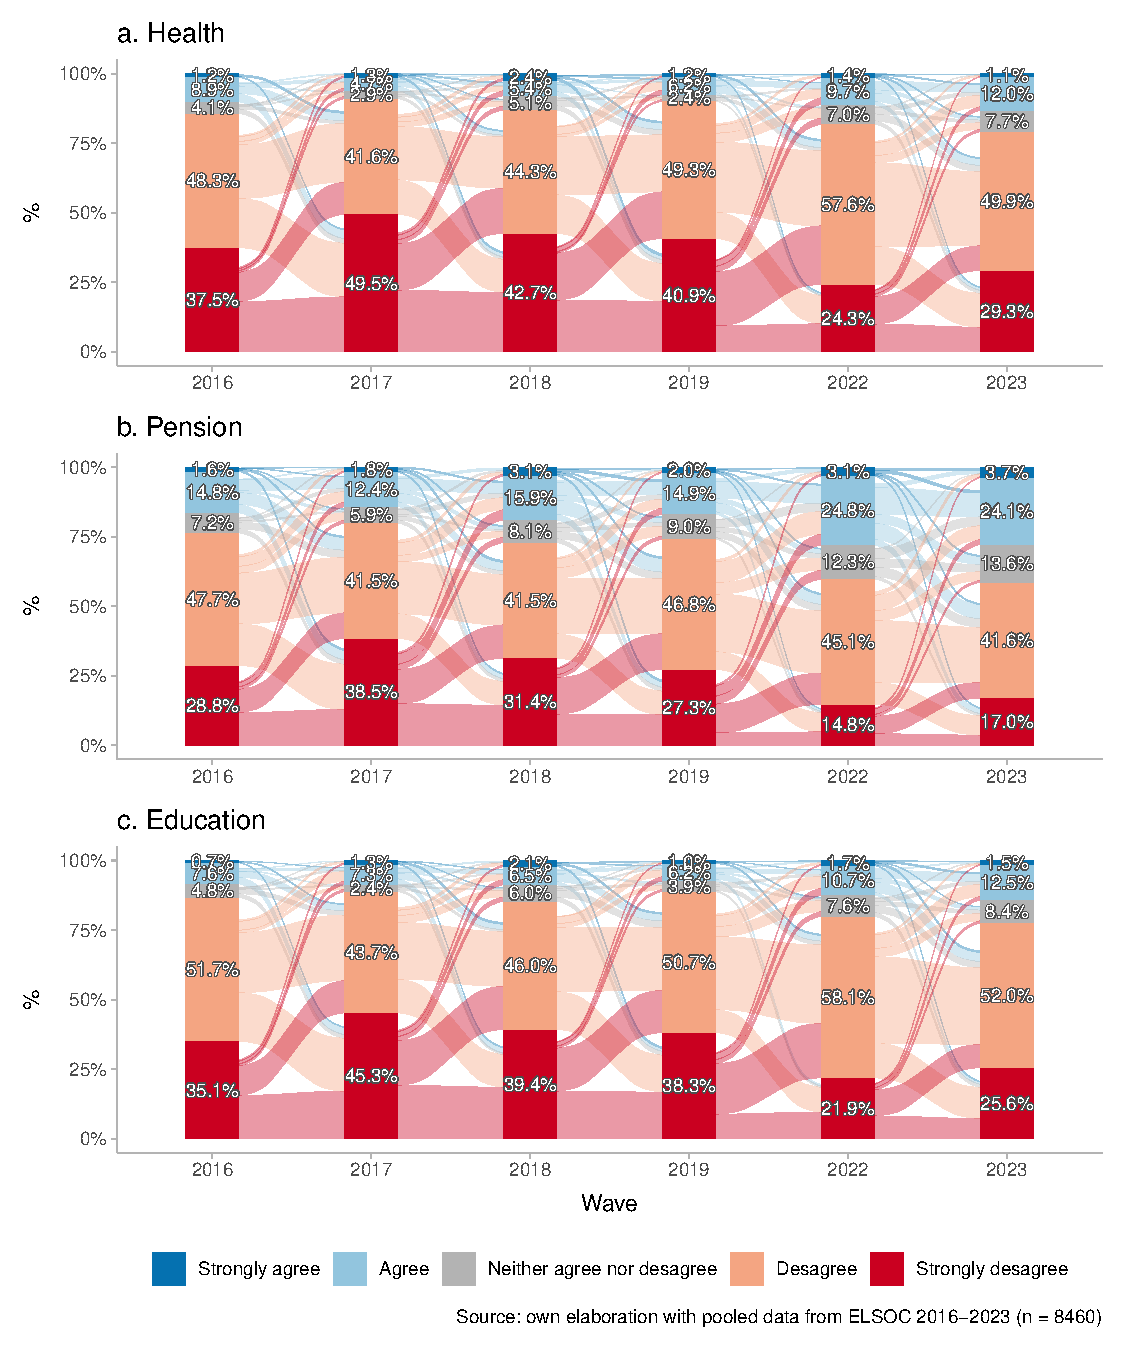
\includegraphics[width=1\textwidth,height=\textheight]{paper_files/figure-pdf/fig-alluvial-1.pdf}

}

\end{figure}%

Regarding the main variables of this study, Figure~\ref{fig-meanchange}
depicts their average changes over the years. We observe an increase in
the average level of market justice preferences in the most recent
waves, which begins in 2019. The highest average consistently appears
for perceived economic inequality, although this variable shows a
downward trend of roughly one point over time. Interestingly, while
perceptions of economic inequality declined in the latest measurements
(2022--2023), market justice preferences increased. With respect to
economic inequality justification, there is a steady decrease in average
levels over the years, registering the lowest mean compared to the other
variables. The meritocracy measures remain stable, though the perception
that individuals are rewarded for intelligence is slightly higher than
the perception that they are rewarded for their effort.

\begin{figure}[H]

\caption{\label{fig-meanchange}Change in the mean of market justice
preferences, economic inequality perception and justification, and
meritocracy (2016-2023)}

\centering{

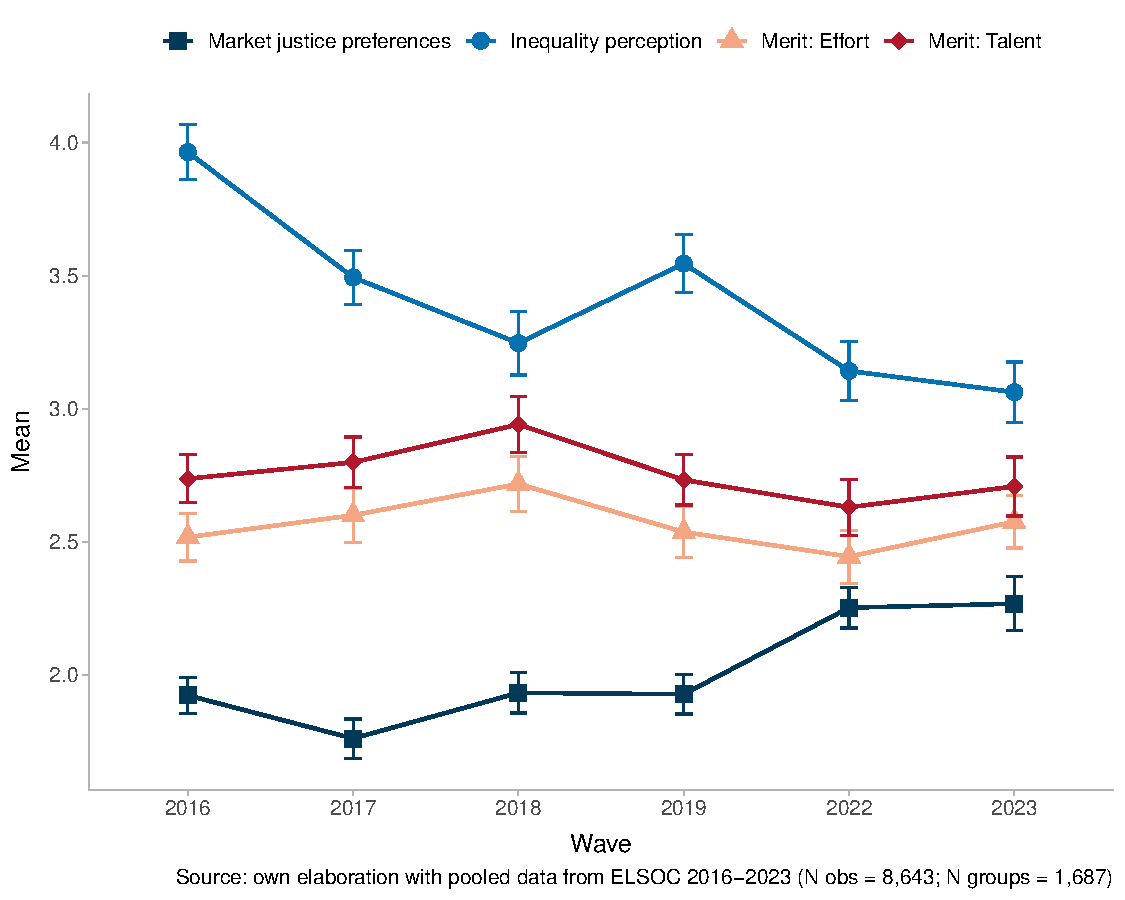
\includegraphics[width=1\textwidth,height=\textheight]{paper_files/figure-pdf/fig-meanchange-1.pdf}

}

\end{figure}%

Figure~\ref{fig-matrix} presents the correlation matrix for the main
variables in the latest wave (2023). Overall, the coefficients range
from low to moderate. The association between market justice preferences
and economic inequality perception is negative but small and not
statistically significant (\(r\) = -0.05, \(p\) \textgreater{} .05). By
contrast, market justice preferences positively and significantly
correlate with the justification of economic inequality (\(r\) = 0.16,
\(p\) \textless{} .01), as well as show low, positive associations with
the two meritocracy variables (\(r\) = 0.14, \(p\) \textless{} .01;
\(r\) = 0.12, \(p\) \textless{} .01). Perceived economic inequality has
a strong, positive correlation with justifying economic inequality
(\(r\) = 0.53, \(p\) \textless{} .01), but negative and nonsignificant
correlations with both meritocracy perceptions (\(r\) = -0.04, \(p\)
\textgreater{} .05; \(r\) = -0.04, \(p\) \textgreater{} .05). The
justification of economic inequality indicator also has small yet
statistically significant positive correlations with the meritocracy
variables (\(r\) = 0.05, \(p\) \textless{} .05; \(r\) = 0.07, \(p\)
\textless{} .01). Finally, the two meritocracy variables exhibit a
strong positive association with each other (\(r\) = 0.69, \(p\)
\textless{} .01).

\begin{figure}[H]

\caption{\label{fig-matrix}Correlation matrix of the main variables for
the last wave (2023)}

\centering{

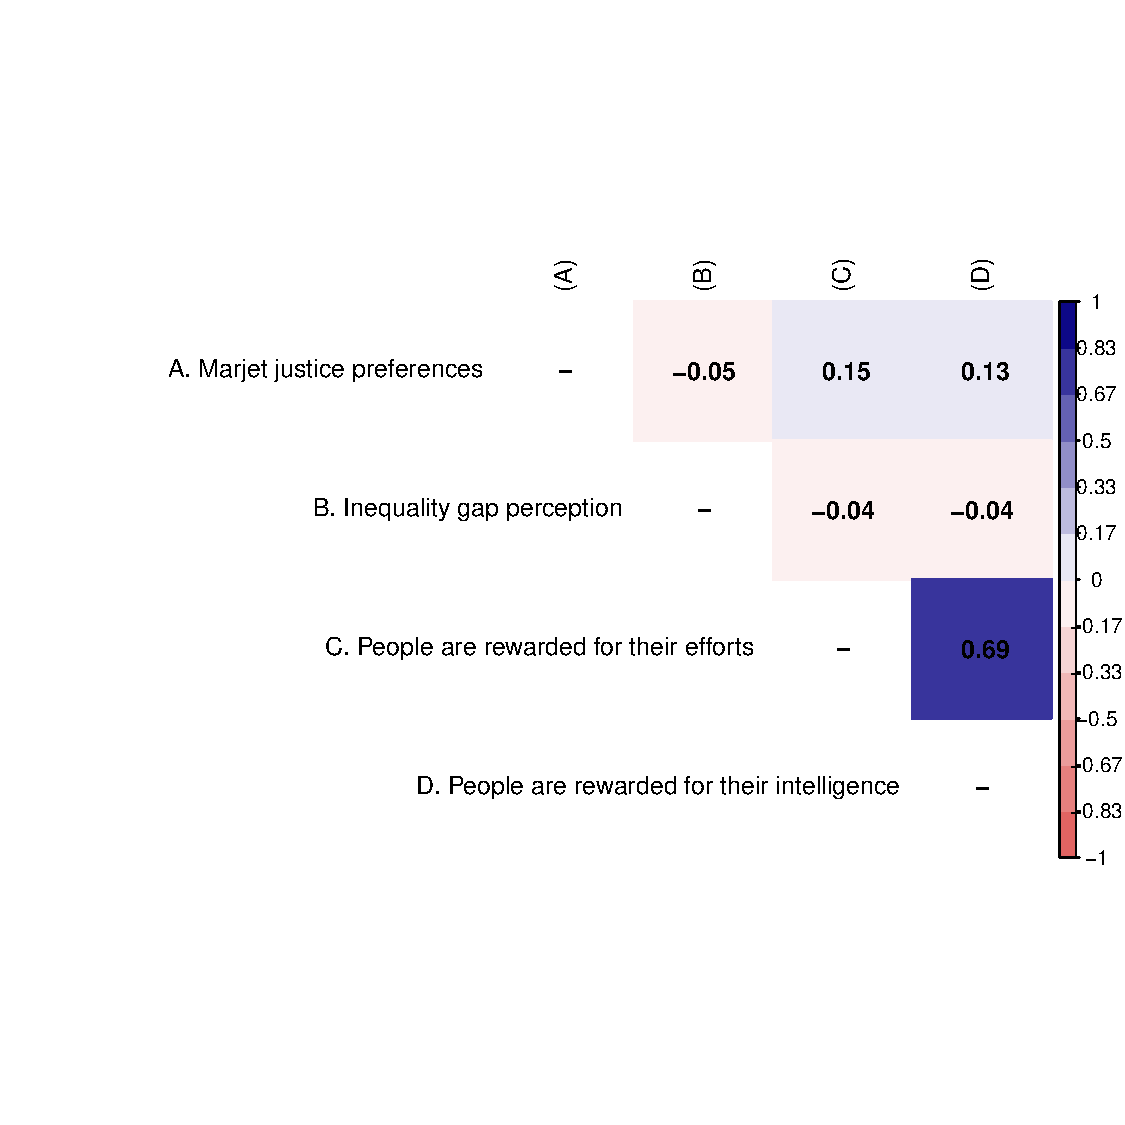
\includegraphics[width=1\textwidth,height=\textheight]{paper_files/figure-pdf/fig-matrix-1.pdf}

}

\end{figure}%

\subsection{Multilevel models}\label{multilevel-models}

Table~\ref{tbl-modelos} presents the results of the multilevel models
estimated for market justice preferences, examining both individuals
(within) and group-level (between) effects. The intraclass correlation
(ICC,
\citeproc{ref-hoxMultilevelAnalysisTechniques2017}{\textbf{hoxMultilevelAnalysisTechniques2017?}})
from the empty model (see Supplementary Material), which decomposes the
variance of market justice preferences, is 0.23, indicating that
approximately 23\% of the variation is attributable to differences
between individuals. Complementary, 77\% of the variation corresponds to
within-individual differences over time.

According to Model 1, which includes the survey waves to capture
intertemporal variations in the dependent variable, there is a decrease
in 2017 (\(\beta\) = -0.162, \(p\) \textless{} .001) relative to 2016,
and similarly in 2018 (\(\beta\) = -0.015, \(p\) \textgreater{} .05) and
2019 (\(\beta\) = -0.041, \(p\) \textgreater{} .05), although the latter
effects are not statistically significant. In contrast, in the more
recent waves of 2022 and 2023, there is a statistically significant
increase in market justice preferences (\(\beta\) = 0.289, \(p\)
\textless{} .001; \(\beta\) = 0.286, \(p\) \textless{} .001), suggesting
a non-linear effect. To model this trajectory over time, Model 2
incorporates time (survey waves) as a continuous variable, along with
its quadratic term, representing the non-linear association initially
observed in Model 1. While the linear term (survey wave) shows a
negative association, reflecting an overall decline in market
preferences over time, the positive quadratic term indicates a reversal
of this pattern in the final measurement points.

\begin{table}

\caption{\label{tbl-modelos}Longitudinal multilevel models for market
justice preferences}

\centering{

[H]
\begin{center}
\scalebox{1}{
\begin{threeparttable}
\begin{tabular}{l c c c c c c c c}
\toprule
 & Model 1 & Model 2 & Model 3 & Model 4 & Model 5 & Model 6 & Model 7 & Model 8 \\
\midrule
Intercept                            & $1.964^{***}$  & $1.966^{***}$  & $2.103^{***}$  & $2.059^{***}$  & $1.752^{***}$  & $1.721^{***}$  & $1.541^{***}$  & $1.574^{***}$  \\
                                     & $(0.022)$      & $(0.033)$      & $(0.046)$      & $(0.045)$      & $(0.052)$      & $(0.053)$      & $(0.095)$      & $(0.112)$      \\
Wave (Ref.= 2016)                    &                &                &                &                &                &                &                &                \\
                                     &                &                &                &                &                &                &                &                \\
\quad Wave 2017                      & $-0.162^{***}$ &                &                &                &                &                &                &                \\
                                     & $(0.028)$      &                &                &                &                &                &                &                \\
\quad Wave 2018                      & $-0.015$       &                &                &                &                &                &                &                \\
                                     & $(0.027)$      &                &                &                &                &                &                &                \\
\quad Wave 2019                      & $-0.041$       &                &                &                &                &                &                &                \\
                                     & $(0.027)$      &                &                &                &                &                &                &                \\
\quad Wave 2022                      & $0.289^{***}$  &                &                &                &                &                &                &                \\
                                     & $(0.028)$      &                &                &                &                &                &                &                \\
\quad Wave 2023                      & $0.286^{***}$  &                &                &                &                &                &                &                \\
                                     & $(0.027)$      &                &                &                &                &                &                &                \\
Wave                                 &                & $-0.069^{***}$ & $-0.072^{***}$ & $-0.057^{**}$  & $-0.057^{**}$  & $-0.058^{**}$  & $-0.064^{***}$ & $-0.064^{***}$ \\
                                     &                & $(0.018)$      & $(0.018)$      & $(0.018)$      & $(0.018)$      & $(0.018)$      & $(0.018)$      & $(0.018)$      \\
Wave$^2$                             &                & $0.017^{***}$  & $0.017^{***}$  & $0.015^{***}$  & $0.015^{***}$  & $0.015^{***}$  & $0.016^{***}$  & $0.016^{***}$  \\
                                     &                & $(0.002)$      & $(0.002)$      & $(0.002)$      & $(0.002)$      & $(0.002)$      & $(0.002)$      & $(0.002)$      \\
Perception inequality (WE)           &                &                & $-0.037^{***}$ & $-0.086^{***}$ & $-0.075^{***}$ & $-0.074^{***}$ & $-0.056^{***}$ & $-0.056^{***}$ \\
                                     &                &                & $(0.009)$      & $(0.010)$      & $(0.010)$      & $(0.010)$      & $(0.011)$      & $(0.011)$      \\
Justification inequality (WE)        &                &                &                & $0.100^{***}$  & $0.095^{***}$  & $0.094^{***}$  & $0.055^{***}$  & $0.055^{***}$  \\
                                     &                &                &                & $(0.009)$      & $(0.009)$      & $(0.009)$      & $(0.010)$      & $(0.010)$      \\
Merit: Effort (WE)                   &                &                &                &                & $0.107^{***}$  & $0.088^{***}$  & $0.071^{***}$  & $0.071^{***}$  \\
                                     &                &                &                &                & $(0.009)$      & $(0.011)$      & $(0.012)$      & $(0.012)$      \\
Merit: Talent (WE)                   &                &                &                &                &                & $0.029^{*}$    & $0.025^{*}$    & $0.025^{*}$    \\
                                     &                &                &                &                &                & $(0.011)$      & $(0.012)$      & $(0.012)$      \\
Perception inequality (BE)           &                &                &                &                &                &                & $-0.077^{***}$ & $-0.078^{***}$ \\
                                     &                &                &                &                &                &                & $(0.023)$      & $(0.023)$      \\
Justification inequality (BE)        &                &                &                &                &                &                & $0.156^{***}$  & $0.131^{***}$  \\
                                     &                &                &                &                &                &                & $(0.021)$      & $(0.021)$      \\
Merit: Effort (BE)                   &                &                &                &                &                &                & $0.092^{**}$   & $0.088^{**}$   \\
                                     &                &                &                &                &                &                & $(0.033)$      & $(0.033)$      \\
Merit: Talent (BE)                   &                &                &                &                &                &                & $-0.006$       & $-0.016$       \\
                                     &                &                &                &                &                &                & $(0.033)$      & $(0.033)$      \\
\midrule
Controls                             & No             & No             & No             & No             & No             & No             & No             & Yes            \\
AIC                                  & $20273.132$    & $20260.158$    & $20251.351$    & $20140.808$    & $20002.562$    & $20005.214$    & $19957.283$    & $19986.833$    \\
BIC                                  & $20329.477$    & $20309.460$    & $20307.696$    & $20204.196$    & $20072.993$    & $20082.688$    & $20062.929$    & $20191.083$    \\
Log Likelihood                       & $-10128.566$   & $-10123.079$   & $-10117.676$   & $-10061.404$   & $-9991.281$    & $-9991.607$    & $-9963.641$    & $-9964.417$    \\
Num. obs.                            & $8460$         & $8460$         & $8460$         & $8460$         & $8460$         & $8460$         & $8460$         & $8460$         \\
Num. groups: idencuesta              & $1681$         & $1681$         & $1681$         & $1681$         & $1681$         & $1681$         & $1681$         & $1681$         \\
Var: idencuesta (Intercept)          & $0.174$        & $0.214$        & $0.210$        & $0.204$        & $0.179$        & $0.178$        & $0.180$        & $0.172$        \\
Var: Residual                        & $0.528$        & $0.494$        & $0.494$        & $0.493$        & $0.490$        & $0.490$        & $0.488$        & $0.488$        \\
Var: idencuesta ola\_num             & $$             & $0.007$        & $0.007$        & $0.007$        & $0.006$        & $0.006$        & $0.006$        & $0.006$        \\
Cov: idencuesta (Intercept) ola\_num & $$             & $-0.018$       & $-0.017$       & $-0.018$       & $-0.015$       & $-0.015$       & $-0.016$       & $-0.016$       \\
\bottomrule
\end{tabular}
\begin{tablenotes}[flushleft]
\scriptsize{Note: Cells contain regression coefficients with standard errors in parentheses. $^{***}p<0.001$; $^{**}p<0.01$; $^{*}p<0.05$.}
\end{tablenotes}
\end{threeparttable}
}
\caption{}
\label{table:coefficients}
\end{center}

}

\end{table}%

Models 3 to 6 incorporate the within-group effects (WE) of the primary
independent variables, capturing how individual changes in these
variables over time shape the dependent variable. The results in Model 3
suggest that the within effect of perceived economic inequality is
negative and statistically significant (\(p\) \textless{} .001).
Specifically, each one-point increase in an individual's perception of
economic inequality between waves is associated with a 0.037 point
decrease in market justice preferences. By contrast, in Model 4, the
within effect of justifying economic inequality is positive and
significant (\(\beta\) = 0.100, \(p\) \textless{} .001), implying that a
rise in an individual's justification of economic inequality over time
corresponds to higher market justice preferences. Regarding meritocratic
variables, Model 5 indicates that the perception of being rewarded for
effort exerts a positive within effect (\(\beta\) = 0.107, \(p\)
\textless{} .001). Similarly, Model 6 shows that viewing intelligence
and ability (talent) as rewarded is also positively related to market
justice preferences (\(\beta\) = 0.029, \(p\) \textless{} .05). Taken
together, these results suggest that individuals who increasingly
perceive meritocracy---whether through effort or talent---tend to hold
stronger market justice preferences.

When examining the between-group effects (BE) in Model 7, which capture
differences between individuals in the average of the main variables, a
similar pattern emerges. Individuals who perceive higher levels of
economic inequality tend to prefer less market justice (\(\beta\) =
-0.077, \(p\) \textless{} .001), whereas those who justify economic
inequality more strongly exhibit higher market justice preferences
(\(\beta\) = 0.156, \(p\) \textless{} .001). Furthermore, the
meritocratic perception that effort is rewarded has a positive impact on
market justice preferences (\(\beta\) = 0.092, \(p\) \textless{} .05).
By contrast, the perception that talent is rewarded shows a negative
coefficient (\(\beta\) = -0.006), though this relationship is not
statistically significant at the 95\% confidence level.

Model 8 introduces the control variables. The within- and
between-effects of the main predictors retain both their direction and
statistical significance, indicating that the associations are robust to
adjustment. Regarding the controls, belonging to higher household-income
quintiles is associated with stronger market-justice preferences:
individuals in the fourth and fifth quintiles score higher than those in
the bottom quintile (\(\beta\) = 0.093, \(p\) \textless{} .05; \(\beta\)
= 0.147, \(p\) \textless{} .001, respectively). Respondents who did not
report their income also express greater support for market justice
(\(\beta\) = 0.172, \(p\) \textless{} .01). Political orientation
matters as well: compared with those on the left, individuals who place
themselves on the right (\(\beta\) = 0.246, \(p\) \textless{} .001) or
who declare no political position (\(\beta\) = 0.092, \(p\) \textless{}
.01) display higher market-justice preferences. Finally, women exhibit
lower market-justice preferences than men (\(\beta\) = −0.080, \(p\)
\textless{} .01).

\begin{table}

\caption{\label{tbl-interactions}Intereactions for within effects and
time}

\centering{

\begin{verbatim}

\begin{table}[h!]
\begin{center}
\scalebox{1}{
\begin{threeparttable}
\begin{tabular}{l c c c c}
\toprule
 & Model 9 & Model 10 & Model 11 & Model 12 \\
\midrule
Intercept                                    & $1.605^{***}$ & $1.679^{***}$ & $1.425^{***}$ & $1.444^{***}$ \\
                                             & $(0.123)$     & $(0.112)$     & $(0.117)$     & $(0.117)$     \\
Perception inequality (WE) x Wave            & $0.002$       &               &               &               \\
                                             & $(0.004)$     &               &               &               \\
Justification inequality (WE) x Wave         &               & $0.013^{***}$ &               &               \\
                                             &               & $(0.003)$     &               &               \\
Merit: Effort (WE) x Wave                    &               &               & $-0.012^{**}$ &               \\
                                             &               &               & $(0.004)$     &               \\
Merit: Talent (WE) x Wave                    &               &               &               & $-0.010^{*}$  \\
                                             &               &               &               & $(0.004)$     \\
\midrule
Controls                                     & Yes           & Yes           & Yes           & Yes           \\
AIC                                          & $19995.908$   & $19923.216$   & $19940.577$   & $19932.452$   \\
BIC                                          & $20228.331$   & $20155.638$   & $20172.999$   & $20164.875$   \\
Log Likelihood                               & $-9964.954$   & $-9928.608$   & $-9937.289$   & $-9933.226$   \\
Num. obs.                                    & $8460$        & $8460$        & $8460$        & $8460$        \\
Num. groups: idencuesta                      & $1681$        & $1681$        & $1681$        & $1681$        \\
Var: idencuesta (Intercept)                  & $0.305$       & $0.198$       & $0.137$       & $0.123$       \\
Var: idencuesta perc\_inequality             & $0.004$       & $$            & $$            & $$            \\
Var: idencuesta ola\_num                     & $0.007$       & $0.006$       & $0.006$       & $0.006$       \\
Cov: idencuesta (Intercept) perc\_inequality & $-0.026$      & $$            & $$            & $$            \\
Cov: idencuesta (Intercept) ola\_num         & $-0.032$      & $-0.027$      & $-0.002$      & $-0.000$      \\
Cov: idencuesta perc\_inequality ola\_num    & $0.004$       & $$            & $$            & $$            \\
Var: Residual                                & $0.485$       & $0.484$       & $0.472$       & $0.471$       \\
Var: idencuesta just\_inequality             & $$            & $0.010$       & $$            & $$            \\
Cov: idencuesta (Intercept) just\_inequality & $$            & $-0.022$      & $$            & $$            \\
Cov: idencuesta just\_inequality ola\_num    & $$            & $0.007$       & $$            & $$            \\
Var: idencuesta merit\_effort                & $$            & $$            & $0.022$       & $$            \\
Cov: idencuesta (Intercept) merit\_effort    & $$            & $$            & $-0.024$      & $$            \\
Cov: idencuesta merit\_effort ola\_num       & $$            & $$            & $-0.005$      & $$            \\
Var: idencuesta merit\_talent                & $$            & $$            & $$            & $0.021$       \\
Cov: idencuesta (Intercept) merit\_talent    & $$            & $$            & $$            & $-0.023$      \\
Cov: idencuesta merit\_talent ola\_num       & $$            & $$            & $$            & $-0.005$      \\
\bottomrule
\end{tabular}
\begin{tablenotes}[flushleft]
\scriptsize{Note: Cells contain regression coefficients with standard errors in parentheses. $^{***}p<0.001$; $^{**}p<0.01$; $^{*}p<0.05$.}
\end{tablenotes}
\end{threeparttable}
}
\caption{}
\label{table:coefficients}
\end{center}
\end{table}
\end{verbatim}

}

\end{table}%

\section{Discussion}\label{discussion}

\section{Conclusion}\label{conclusion}

\section{References}\label{references}

\phantomsection\label{refs}
\begin{CSLReferences}{1}{0}
\bibitem[\citeproctext]{ref-akyelken_urban_2020}
Akyelken, N. (2020). Urban conceptions of economic inequalities.
\emph{Regional Studies}, \emph{54}(6), 863--872.
\url{https://doi.org/10.1080/00343404.2020.1732902}

\bibitem[\citeproctext]{ref-bates_fitting_2015}
Bates, D., Mächler, M., Bolker, B., \& Walker, S. (2015). Fitting linear
mixed-effects models using {lme4}. \emph{Journal of Statistical
Software}, \emph{67}(1), 1--48.
\url{https://doi.org/10.18637/jss.v067.i01}

\bibitem[\citeproctext]{ref-batruch_belief_2023}
Batruch, A., Jetten, J., Van De Werfhorst, H., Darnon, C., \& Butera, F.
(2023). Belief in {School Meritocracy} and the {Legitimization} of
{Social} and {Income Inequality}. \emph{Social Psychological and
Personality Science}, \emph{14}(5), 621--635.
\url{https://doi.org/10.1177/19485506221111017}

\bibitem[\citeproctext]{ref-boccardo_30_2020}
Boccardo, G. (2020). \emph{30 a{ñ}os de privatizaciones en {Chile}: Lo
que la pandemia revel{ó}} (Nodo XXI). Santiago.

\bibitem[\citeproctext]{ref-Castillo2011}
Castillo, J. C. (2011). Legitimacy of {Inequality} in a {Highly Unequal
Context}: {Evidence} from the {Chilean Case}. \emph{Social Justice
Research}, \emph{24}(4), 314--340.
\url{https://doi.org/10.1007/s11211-011-0144-5}

\bibitem[\citeproctext]{ref-castillo_perception_2022}
Castillo, J. C., García-Castro, J.-D., \& Venegas, M. (2022). Perception
of economic inequality: Concepts, associated factors and prospects of a
burgeoning research agenda. \emph{International Journal of Social
Psychology}, \emph{37}(1), 180--207.
\url{https://doi.org/10.1080/02134748.2021.2009275}

\bibitem[\citeproctext]{ref-castillo_multidimensional_2023}
Castillo, J. C., Iturra, J., Maldonado, L., Atria, J., \& Meneses, F.
(2023). A {Multidimensional Approach} for {Measuring Meritocratic
Beliefs}: {Advantages}, {Limitations} and {Alternatives} to the {ISSP
Social Inequality Survey}. \emph{International Journal of Sociology},
1--25. \url{https://doi.org/10.1080/00207659.2023.2274712}

\bibitem[\citeproctext]{ref-castillo_percepcion_2019}
Castillo, J. C., Miranda, D., \& Carrasco, D. (2012). Percepci{ó}n de
{Desigualdad Econ{ó}mica} en {Chile}: {Medici{ó}n}, {Diferencias} y
{Determinantes}. \emph{Psykhe (Santiago)}, \emph{21}(1), 99--114.
\url{https://doi.org/10.4067/S0718-22282012000100007}

\bibitem[\citeproctext]{ref-castillo_socialization_2024}
Castillo, J. C., Salgado, M., Carrasco, K., \& Laffert, A. (2024). The
{Socialization} of {Meritocracy} and {Market Justice Preferences} at
{School}. \emph{Societies}, \emph{14}(11), 214.
\url{https://doi.org/10.3390/soc14110214}

\bibitem[\citeproctext]{ref-chancel_world_2022}
Chancel, L., Piketty, T., Saez, E., \& Zucman, G. (2022). World
inequality report 2022.
https://bibliotecadigital.ccb.org.co/handle/11520/27510.

\bibitem[\citeproctext]{ref-davis_principles_2001}
Davis, K., \& Moore, W. E. (2001). Some {Principles} of
{Stratification}. In \emph{Social {Stratification}, {Class}, {Race}, and
{Gender} in {Sociological Perspective}, {Second Edition}} (2nd ed.).
Routledge.

\bibitem[\citeproctext]{ref-easterbrook_social_2021}
Easterbrook, M. J. (2021). \emph{The social psychology of economic
inequality} (43rd ed., Vol. 2021). UNU-WIDER.
\url{https://doi.org/10.35188/UNU-WIDER/2021/981-5}

\bibitem[\citeproctext]{ref-elsoc_estudio_2022}
ELSOC, S. T. (2022). Estudio {Longitudinal Social} de {Chile}. Harvard
Dataverse. \url{https://doi.org/10.7910/dvn/0kirbj}

\bibitem[\citeproctext]{ref-engelhardt_what_2018}
Engelhardt, C., \& Wagener, A. (2018). What do {Germans} think and know
about income inequality? {A} survey experiment. \emph{Socio-Economic
Review}, \emph{16}(4), 743--767.
\url{https://doi.org/10.1093/ser/mwx036}

\bibitem[\citeproctext]{ref-flores_top_2020}
Flores, I., Sanhueza, C., Atria, J., \& Mayer, R. (2020). Top {Incomes}
in {Chile}: {A Historical Perspective} on {Income Inequality},
1964--2017. \emph{Review of Income and Wealth}, \emph{66}(4), 850--874.
\url{https://doi.org/10.1111/roiw.12441}

\bibitem[\citeproctext]{ref-garcia-castro_perceiving_2020}
García-Castro, J. D., Rodríguez-Bailón, R., \& Willis, G. B. (2020).
Perceiving economic inequality in everyday life decreases tolerance to
inequality. \emph{Journal of Experimental Social Psychology}, \emph{90},
104019. \url{https://doi.org/10.1016/j.jesp.2020.104019}

\bibitem[\citeproctext]{ref-garcia-sanchez_creencias_2022}
García-Sánchez, E., \& De Carvalho, S. (2022). Las creencias que
justifican la desigualdad moderan la relaci{ó}n entre el estatus
socioecon{ó}mico y el apoyo a la redistribuci{ó}n. \emph{Revista
Internacional de Sociolog{í}a}, \emph{80}(3), e210.
\url{https://doi.org/10.3989/ris.2022.80.3.21.29}

\bibitem[\citeproctext]{ref-garcia-sanchez_vicious_2019}
García-Sánchez, E., Van Der Toorn, J., Rodríguez-Bailón, R., \& Willis,
G. B. (2019). The {Vicious Cycle} of {Economic Inequality}: {The Role}
of {Ideology} in {Shaping} the {Relationship Between} {``{What Is}''}
and {``{What Ought} to {Be}''} in 41 {Countries}. \emph{Social
Psychological and Personality Science}, \emph{10}(8), 991--1001.
\url{https://doi.org/10.1177/1948550618811500}

\bibitem[\citeproctext]{ref-garcia-sanchez_perceptions_2018}
García-Sánchez, E., Willis, G. B., Rodríguez-Bailón, R., Palacio Sañudo,
J., David Polo, J., \& Rentería Pérez, E. (2018). Perceptions of
{Economic Inequality} and {Support} for {Redistribution}: {The} role of
{Existential} and {Utopian Standards}. \emph{Social Justice Research},
\emph{31}(4), 335--354. \url{https://doi.org/10.1007/s11211-018-0317-6}

\bibitem[\citeproctext]{ref-gimpelson_misperceiving_2018}
Gimpelson, V., \& Treisman, D. (2018). Misperceiving inequality.
\emph{Economics \& Politics}, \emph{30}(1), 27--54.
\url{https://doi.org/10.1111/ecpo.12103}

\bibitem[\citeproctext]{ref-immergut_it_2020}
Immergut, E. M., \& Schneider, S. M. (2020). Is it unfair for the
affluent to be able to purchase {``better''} healthcare? {Existential}
standards and institutional norms in healthcare attitudes across 28
countries. \emph{Social Science \& Medicine}, \emph{267}, 113146.
\url{https://doi.org/10.1016/j.socscimed.2020.113146}

\bibitem[\citeproctext]{ref-janmaat_subjective_2013}
Janmaat, J. G. (2013). Subjective inequality: {A} review of
international comparative studies on people's views about inequality.
\emph{Archives Europeennes de Sociologie}, \emph{54}(3), 357--389.
\url{https://doi.org/10.1017/S0003975613000209}

\bibitem[\citeproctext]{ref-kluegel_social_1995a}
Kluegel, J. R., Mason, D. S., \& Wegener, B. (Eds.). (1995).
\emph{Social {Justice} and {Political Change}: {Public Opinion} in
{Capitalist} and {Post-Communist States}} (1st ed.). Routledge.

\bibitem[\citeproctext]{ref-kluegel_legitimation_1999}
Kluegel, J. R., Mason, D. S., \& Wegener, B. (1999). The {Legitimation}
of {Capitalism} in the {Postcommunist Transition}: {Public Opinion}
about {Market Justice}, 1991-1996. \emph{European Sociological Review},
\emph{15}(3), 251--283. Retrieved from
\url{https://www.jstor.org/stable/522731}

\bibitem[\citeproctext]{ref-kluegel_beliefs_1981}
Kluegel, J. R., \& Smith, E. R. (1981). Beliefs {About Stratification}.
\emph{Annual Review of Sociology}, 29--56.

\bibitem[\citeproctext]{ref-knell_perceptions_2020}
Knell, M., \& Stix, H. (2020). Perceptions of inequality. \emph{European
Journal of Political Economy}, \emph{65}, 101927.
\url{https://doi.org/10.1016/j.ejpoleco.2020.101927}

\bibitem[\citeproctext]{ref-koos_moral_2019}
Koos, S., \& Sachweh, P. (2019). The moral economies of market
societies: Popular attitudes towards market competition, redistribution
and reciprocity in comparative perspective. \emph{Socio-Economic
Review}, \emph{17}(4), 793--821.
\url{https://doi.org/10.1093/ser/mwx045}

\bibitem[\citeproctext]{ref-kuhn_eye_2011}
Kuhn, A. (2011). In the eye of the beholder: {Subjective} inequality
measures and individuals' assessment of market justice. \emph{European
Journal of Political Economy}, \emph{27}(4), 625--641.
\url{https://doi.org/10.1016/j.ejpoleco.2011.06.002}

\bibitem[\citeproctext]{ref-lane_market_1986}
Lane, R. E. (1986). Market {Justice}, {Political Justice}.
\emph{American Political Science Review}, \emph{80}(2), 383--402.
\url{https://doi.org/10.2307/1958264}

\bibitem[\citeproctext]{ref-lee_fairness_2023}
Lee, J.-S., \& Stacey, M. (2023). Fairness perceptions of educational
inequality: The effects of self-interest and neoliberal orientations.
\emph{The Australian Educational Researcher}.
\url{https://doi.org/10.1007/s13384-023-00636-6}

\bibitem[\citeproctext]{ref-lindh_public_2015}
Lindh, A. (2015). Public {Opinion} against {Markets}? {Attitudes}
towards {Market Distribution} of {Social Services} -- {A Comparison} of
17 {Countries}. \emph{Social Policy \& Administration}, \emph{49}(7),
887--910. \url{https://doi.org/10.1111/spol.12105}

\bibitem[\citeproctext]{ref-mijs_stratified_2016}
Mijs, J. (2016). Stratified {Failure}: {Educational Stratification} and
{Students}' {Attributions} of {Their Mathematics Performance} in 24
{Countries}. \emph{Sociology of Education}, \emph{89}(2), 137--153.
\url{https://doi.org/10.1177/0038040716636434}

\bibitem[\citeproctext]{ref-mijs_paradox_2021}
Mijs, J. (2021). The paradox of inequality: Income inequality and belief
in meritocracy go hand in hand. \emph{Socio-Economic Review},
\emph{19}(1), 7--35. \url{https://doi.org/10.1093/ser/mwy051}

\bibitem[\citeproctext]{ref-pedersen_attitudes_2019}
Pedersen, R. T., \& Mutz, D. C. (2019). Attitudes {Toward Economic
Inequality}: {The Illusory Agreement}. \emph{Political Science Research
and Methods}, \emph{7}(04), 835--851.
\url{https://doi.org/10.1017/psrm.2018.18}

\bibitem[\citeproctext]{ref-reynolds_perceptions_2014}
Reynolds, J., \& Xian, H. (2014). Perceptions of meritocracy in the land
of opportunity. \emph{Research in Social Stratification and Mobility},
\emph{36}, 121--137. \url{https://doi.org/10.1016/j.rssm.2014.03.001}

\bibitem[\citeproctext]{ref-sandel_tyranny_2020}
Sandel, M. J. (2020). \emph{The tyranny of merit: {What}'s become of the
common good?} (First edition). New York: {Farrar, Straus and Giroux}.

\bibitem[\citeproctext]{ref-schneider_poverty_2015}
Schneider, S. M., \& Castillo, J. C. (2015). Poverty {Attributions} and
the {Perceived Justice} of {Income Inequality} : {A Comparison} of
{East} and {West Germany}.
\url{https://doi.org/10.1177/0190272515589298}

\bibitem[\citeproctext]{ref-schroder_income_2017}
Schröder, M. (2017). Is {Income Inequality Related} to {Tolerance} for
{Inequality}? \emph{Social Justice Research}, \emph{30}(1), 23--47.
\url{https://doi.org/10.1007/s11211-016-0276-8}

\bibitem[\citeproctext]{ref-singer_applied_2009}
Singer, J. D., \& Willett, J. B. (2009). \emph{Applied longitudinal data
analysis: Modeling change and event occurence}. New York: Oxford
University Press, Incorporated.

\bibitem[\citeproctext]{ref-svallfors_political_2007}
Svallfors, S. (Ed.). (2007). \emph{The {Political Sociology} of the
{Welfare State}: {Institutions}, {Social Cleavages}, and {Orientations}}
(1st ed.). Stanford University Press.
\url{https://doi.org/10.2307/j.ctvr0qv0q}

\bibitem[\citeproctext]{ref-trump_income_2018}
Trump, K.-S. (2018). Income {Inequality Influences Perceptions} of
{Legitimate Income Differences}. \emph{British Journal of Political
Science}, \emph{48}(4), 929--952.
\url{https://doi.org/10.1017/S0007123416000326}

\bibitem[\citeproctext]{ref-wilson_role_2003}
Wilson, C. (2003). The {Role} of a {Merit Principle} in {Distributive
Justice}. \emph{The Journal of Ethics}, \emph{7}(3), 277--314.
\url{https://doi.org/10.1023/A:1024667228488}

\bibitem[\citeproctext]{ref-young_rise_1962}
Young, M. (1962). \emph{The rise of the meritocracy}. Baltimore: Penguin
Books.

\end{CSLReferences}



\end{document}
